%%%%%%%%%%%%%%%%%%%%%%%%%%%%%%%%%%%%%%%%%%%%%%%%%%%%%%%%%%%%%%%%%%%%%%%%%%%%%%%
%% Active Learning Machine Learning Results
%%
%%%%%%%%%%%%%%%%%%%%%%%%%%%%%%%%%%%%%%%%%%%%%%%%%%%%%%%%%%%%%%%%%%%%%%%%%%%%%%%


% #############################################################################
% #############################################################################
% ██████  ███████ ███████ ██    ██ ██   ████████ ███████
% ██   ██ ██      ██      ██    ██ ██      ██    ██
% ██████  █████   ███████ ██    ██ ██      ██    ███████
% ██   ██ ██           ██ ██    ██ ██      ██         ██
% ██   ██ ███████ ███████  ██████  ███████ ██    ███████
% #############################################################################
% #############################################################################
% Notes:
%   - QUESTION Is there any physical intuition that we can gleam from the fingerprints?
%   - QUESTION What did @Chris mean by this? "Computed amorphous phase to define synthesizability"
% #############################################################################
% #############################################################################



% ################################# Paragraph #################################
% %%%%%%%%%%%%%%%%%%%%%%%%%%%%%%%%%%%%%%%%%%%%%%%%%%%%%%%%%%%%%%%%%%%%%%%%%%%%%
% Intro/transition paragraph
%
% %%%%%%%%%%%%%%%%%%%%%%%%%%%%%%%%%%%%%%%%%%%%%%%%%%%%%%%%%%%%%%%%%%%%%%%%%%%%%
% | - Paragraph start
%
We now turn our attention of the application of this active learning scheme to the discovery of stable forms of IrO2 and IrO3.
% Comment on this line | TODO do stuff
%The AL algorithm is applied separately to IrO2 and IrO3 because we are specifically interested in the most stable polymorphs at each stoichiometry.
% TODO How many features drop out when you constrain the stoich.?
%This has an the added benefit of reducing the number of fingerprint vectors from the Voronoi tesselation dramatically (from TEMP to TEMP) because many features are senstive to changes in stoicheometry.
% __|
% ################################# Paragraph #################################
% %%%%%%%%%%%%%%%%%%%%%%%%%%%%%%%%%%%%%%%%%%%%%%%%%%%%%%%%%%%%%%%%%%%%%%%%%%%%%
% Results for IrO3
% MAIN RESULTS:
%   How many generations to find top 2-3 structures?
% We need to call them something else than "convergence plots" (bad name)
% %%%%%%%%%%%%%%%%%%%%%%%%%%%%%%%%%%%%%%%%%%%%%%%%%%%%%%%%%%%%%%%%%%%%%%%%%%%%%
% | - Paragraph start
%
Figure \ref{fig:iro2_al} a and b shows several iterations of the active learning loop for the IrO3 candidate space. 
An acquisition bin size of 10 DFT calculations per iteration and an initial seed of 11 calculations were used.
%plots of the AL predictions on the candidate space at particular generations of the AL algorithm for the IrO3 candidate space with an aquisition bin size of 10 DFT calculations per iteration and an initial 11 calculations used for seeding.
%
Figure \ref{fig:iro2_al} a. shows the progression of the model at selected generations of the active learning loop.
%
As seen from Figure\ref{fig:iro2_al} a) the early iterations, where the training data is sparse 
%
Figure \ref{fig:iro2_al} b. shows the formation energy, either predicted (small colored circles) or computed (large red-bordered circles), is plotted on the y-axis against all structures in the candidate space of IrO3 polymorphs.
%
The DFT derived formation energy is plotted alongside the predicted data (hollow diamonds).
%
It is evident from figure \ref{fig:iro2_al}, that the Gaussian process model is doing a poor job of predicting the DFT formation energy of the candidate space, with a exceptionally poor MAE of TEMP eV/atom at the AL generation shown here.
%
This is significantly lower than the leave-one out cross validation error of TEMP ~0.15 eV/atom, which indicates that the issue does not lie with a poor predictive model.
%
Instead, the issue lies with the large degree of structural reorganization that occurs over the course of a typical DFT ionic optimization.
% TODO Change wording when @Kirsten uses the protosearch to optimize candidates
% UPDATE | Using protosearch pre-optimizer isn't worth it, no siginificant improvement
%Because the candidate space structures are generated
% To compare the performance of the AL routine we compare against a
%
Figure subplot TEMP shows the parity plot of the predicted DFT energies using the fingerprints corresponding to the unoptimized structures (COLOR1) and post-DFT relaxed structures (COLOR2),
plotted against the final post-optimization DFT formation energy.
% Sentence that explains the parity plot
It is clear that the GP model severely underpredicts the energy of the candidate space, especially for systems with less stable predicted formation energies, when predicting onto the candidate space of unoptimized structures (MAE of ~0.5 eV/atom).
%
This is due to the fact that the structures undergo through a large degree of structural rearrangement over the course of the DFT relaxation.
%
Alternatively, the MAE is much lower when the model predicts onto the post-optimized structures (MAE ~0.15 eV/atom),
demonstrating that the poor preditive capabilities is due primarily to structural drift and not to the poor predictive capabilities of the GP model.
%
Despite these shortcomings, figure TEMP (TEMP performance plot) tracks the number of high stability materials (lowest N structures) discovered as a function of the number of DFT calculations for the case of 1.) AL with UCB acquisition function and 2.) AL with a random acquisition function.
%
The random acquisition function emulates the behavior of regression model which exhibits no correlation between the input and output space.
%
Clearly, the rate of discovery for case 1.) is superior to that of case 2.), with our methodology discovering half of the lowest N structures after only TEMP DFT calculations compared to TEMP when acquiring randomley within the candidate space.
% __|


% | - Figure | IrO3 Convergence Plot
\begin{figure*}
\centering
\makebox[\textwidth][c]{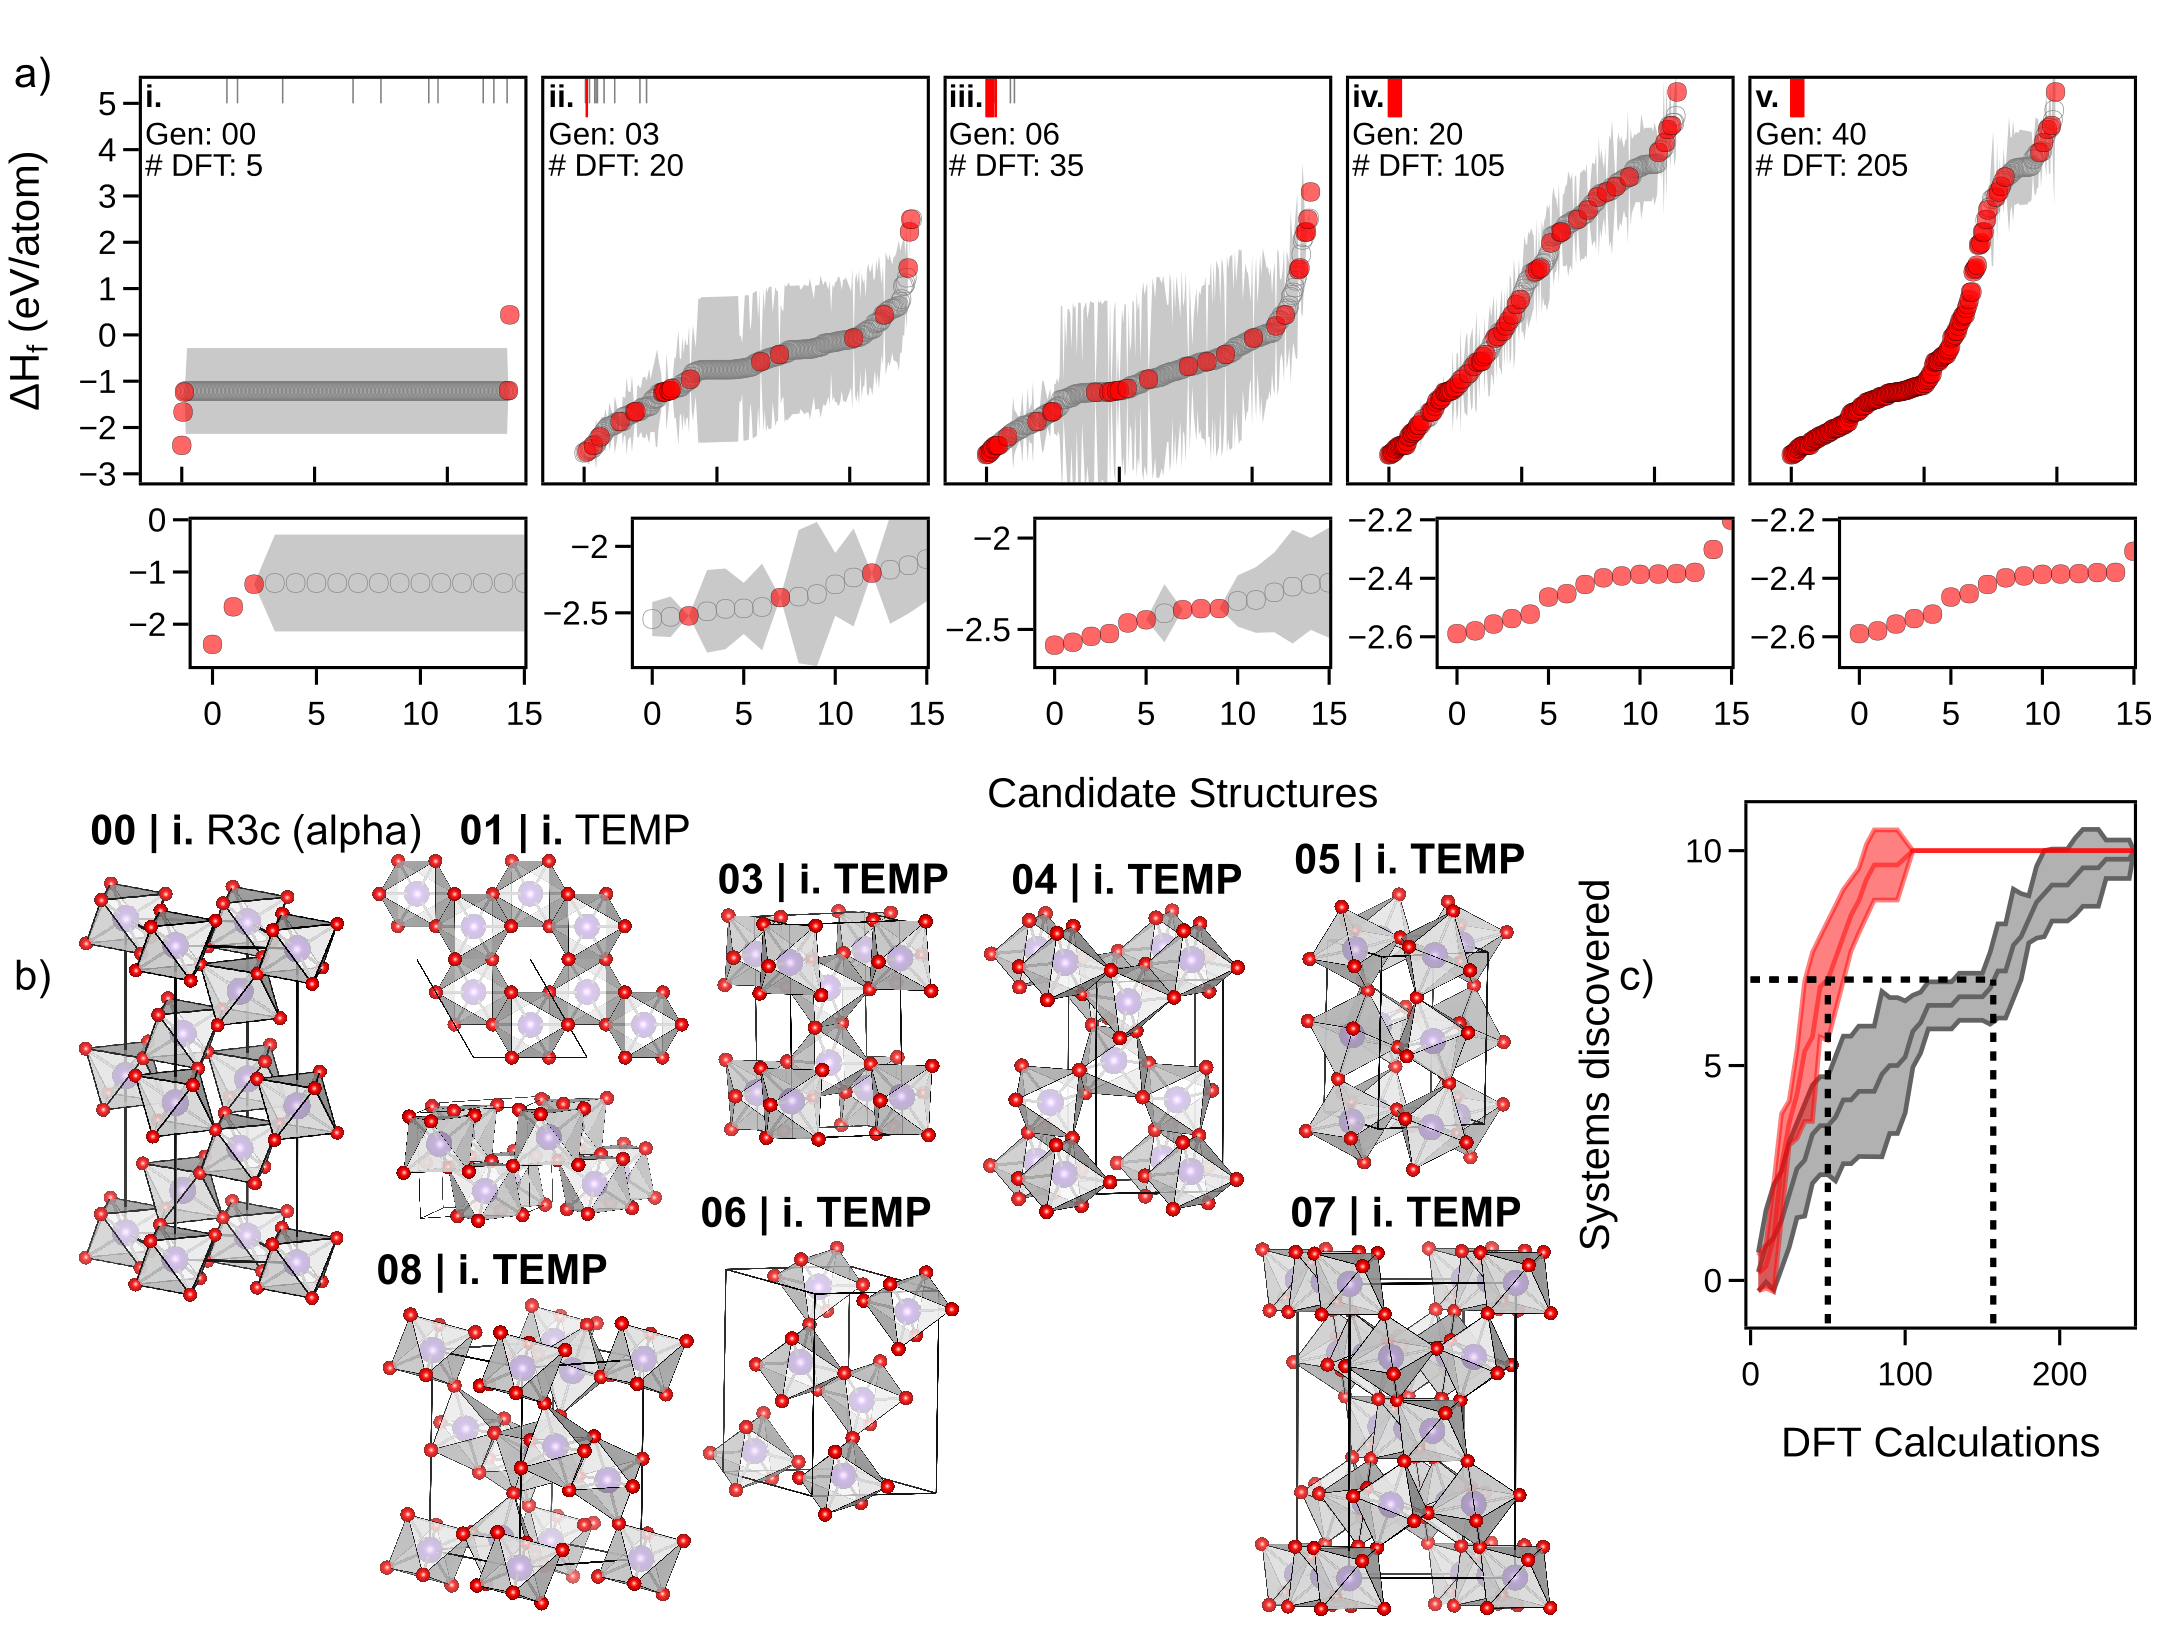
\includegraphics[width=\textwidth,height=\textheight,keepaspectratio]
{02_figures/ml_convergence_plots/test_iro3_al.png}
}
\caption{\label{fig:iro2_al}
Results from machine-learning accelerated active learning material discovery algorithm.
% FORMATION ENTHALPY, FIX
Both (a) and (b) plot the formation enthalpy (either predicted from the model or computed by DFT) for each system in the candidate pool, ordered by decreasing stability (low to high formation energy).
%
Formation energies predicted by the surrogate model are represented by smaller circles,
while acquired DFT formation energies are shown as enlarged red bordered circles.
%
Each data point is colored based on the ordering of the DFT formation energies, with low formation energy systems on the dark end of the spectrum and the highest formation energy species colored light.
%
Error bars representing 1 sigma standard deviation from the Gaussian Process model are shown for each prediction.
%
(a) Series of ML convergence plots at different generations of the active learning algorithm.
%
The middle panel indicates the generation which satisifies the AL stop criteria (see text)
%
(b) Expanded ML plot for the generation that satisfies the stop criteria.
%
Black diamonds indicate the actual DFT formation energy for each system.
%
Inset shows the most stable 20 systems that are within the energetic window of meta-stability (indicated by grey band).
%
(c)
Number of the top 20 polymorphs discovered as a function of the AL generation number for the AL loop using the aquisition criteria in equation TEMP and a control run that utilized a random  aquisition method.


% | - __old__
% Gaussian process machine learning models trained initially on (a) publicly available DFT data for IrO2 and (b) all of the acquired DFT calculations from the active learning algorithm.
% See SI for additional panels at intermediate iterations of the active learning algorithm.
% The Gibbs formation energy (either DFT derived or predicted from the GP model) and associated GP estimated error (2 sigmas or something TEMP) is plotted for each polymorph in the IrO2 candidate space.
% The data points in each subset are ordered from most to least stable (lowest to largest DE formation).
% The individual markers are colored based on their ordering in the final converged GP model.
% Acquired structures are identified by their red borders and slightly larger size.
% The insets show the most stable TEMP structures, where several well known crystal structures are labeled.
% __|

}
\end{figure*}
% __|


% #############################################################################
% | - __old__
% ################################# Paragraph #################################
% AB2 Structures Ankit
% - There are XYZ unique AB2 structures (or multiples, e.g. A2B4)
% - Of those we found 697 unique AB2 prototypes (unique SG/Wyckoff combination) in OQMD/MP
% - To generate our test set we substituted Ir for A and O for B, then isotropically expanded cell volume to constrain a minimum Ir-O distance of XYZ
% - Next translated each of the 697 structures to be described by 271 features (invariant to isotropic expansion/compression), then reduced to 30 using PCA, described in methods XYZ
% - To generate initial training data use existing DFT. Not enough on \ce{IrO_2}, so used OQMD to generate initial training data from nearest structures in phase space, described in Methods XYZ. Training set of 30 structures in SI XYZ.
% __|
